\subsubsection{Wild Pokémon (Headbuttable Trees)}%
\label{ssubsec:WildPokmon(HeadbuttableTrees)}%
\begin{longtable}{||l l l l||}%
\hline%
\rowcolor{GroundColor}%
&Pokémon&Level Range&Rarity Tier\\%
\hline%
\endhead%
\hline%
\rowcolor{GroundColor}%

\includegraphics[width=0.02\textwidth]{pokemon/Bidoof}&Bidoof&35{-}39&\textcolor{black}{%
Common%
}\\%
\hline%
\rowcolor{GroundColor}%

\includegraphics[width=0.02\textwidth]{pokemon/Kricketot}&Kricketot&35{-}39&\textcolor{black}{%
Common%
}\\%
\hline%
\rowcolor{GroundColor}%
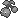
\includegraphics[width=0.02\textwidth]{pokemon/Cherubi}&Cherubi&35{-}39&\textcolor{black}{%
Common%
}\\%
\hline%
\rowcolor{GroundColor}%

\includegraphics[width=0.02\textwidth]{pokemon/Starly}&Starly&35{-}39&\textcolor{black}{%
Common%
}\\%
\hline%
\rowcolor{GroundColor}%

\includegraphics[width=0.02\textwidth]{pokemon/Carnivine}&Carnivine&35{-}39&\textcolor{OliveGreen}{%
Uncommon%
}\\%
\hline%
\rowcolor{GroundColor}%

\includegraphics[width=0.02\textwidth]{pokemon/Pachirisu}&Pachirisu&35{-}39&\textcolor{RedOrange}{%
Rare%
}\\%
\hline%
\end{longtable}%
\caption{Wild Pokemon in Lake Valor (Headbuttable Trees)}